% ============================================================================
% Plain-English version of the Computer Animation report
% Same structure, same data, simpler vocabulary
% ============================================================================
\documentclass[10pt,a4paper,twocolumn]{article}

\usepackage[a4paper, left=15mm, right=15mm, top=20mm, bottom=20mm,
            columnsep=6mm, headheight=12pt]{geometry}
\usepackage[T1]{fontenc}
\usepackage[utf8]{inputenc}
\usepackage[protrusion=true,expansion=false]{microtype}
\usepackage{amsmath,amssymb}
\usepackage{booktabs}
\usepackage{array}
\usepackage{graphicx}
\usepackage{subcaption}
\usepackage{caption}
\captionsetup{font=small, labelfont=bf}
\usepackage{algorithm}
\usepackage{algpseudocode}
\usepackage{xcolor}
\usepackage{url}
\usepackage[hidelinks]{hyperref}
\usepackage{enumitem}
\setlist{nosep,leftmargin=*}

\usepackage{titling}
\setlength{\droptitle}{-1.2cm}
\pretitle{\begin{center}\Large\bfseries}
\posttitle{\par\end{center}\vspace{0.2em}}
\preauthor{\begin{center}\small}
\postauthor{\par\end{center}\vspace{-0.5em}}
\predate{\begin{center}\small\itshape}
\postdate{\par\end{center}\vspace{-0.5em}}

\usepackage{titlesec}
\titleformat{\section}{\normalfont\bfseries\large}{\Roman{section}.}{0.5em}{}
\titleformat{\subsection}{\normalfont\bfseries}{\Alph{subsection}.}{0.5em}{\itshape}
\titlespacing*{\section}{0pt}{0.8em}{0.4em}
\titlespacing*{\subsection}{0pt}{0.5em}{0.2em}

\setlength{\textfloatsep}{6pt}
\setlength{\floatsep}{6pt}
\setlength{\intextsep}{6pt}
\setlength{\abovecaptionskip}{4pt}
\setlength{\belowcaptionskip}{2pt}

\renewenvironment{abstract}{%
  \par\noindent\textbf{\textit{Abstract---}}\itshape\small\ignorespaces}
  {\par\vspace{0.3em}}
\newcommand{\keywords}[1]{\par\noindent\textbf{\textit{Keywords---}}\textit{#1}\par\vspace{0.5em}}

\title{Collision-Aware Chaikin's Algorithm:\\
       Smoothing Paths Around Obstacles for\\
       Real-Time 2D Animation}

\author{Phatorn Pitiphat (6531332121) \quad
        Sukrit Chanachaimongkonkun (6531345321) \quad
        Sathana Laolugsanalerd (6532180221) \\
        Athiwat Kongkaeo (6531347621) \quad
        Chakit Prateepthintong (6531348221) \\
        \small GitHub: \texttt{github.com/sumopht} \\
        \small Department of Computer Engineering, Faculty of Engineering, Chulalongkorn University \\
        \small Computer Animation, Second Semester, Academic Year 2568 \\
        \small Instructor: Assoc.\ Prof.\ Pizzanu Kanongchaiyos, Ph.D.}
\date{}

\begin{document}
\twocolumn[\maketitle
\begin{@twocolumnfalse}
\begin{abstract}
When an animated character walks from one place to another, a path
planner first picks a sequence of waypoints, and then a smoothing
algorithm turns those waypoints into a smooth curve so the character
moves naturally instead of in straight lines. The classical method,
\emph{Chaikin's algorithm}, makes the curve smooth but does not check
for obstacles, so the smoothed curve can cut through walls. We propose
a modified version that combines Chaikin's smoothing with a simple
push-out step: after each smoothing pass, any point that ended up
inside an obstacle is pushed out, and any line segment crossing an
obstacle gets a new midpoint inserted that goes around it. We built an
interactive 2D demo and ran 20 trials on each of three test sizes
(input size $N{=}5$ to $5000$ waypoints, obstacle count $K{=}0$ to $32$,
smoothing rounds $T{=}2$ to $6$). Results: the new method removes all
collisions in $85\%$ of trials when there are few obstacles, but only
$0\%$ when obstacles overlap heavily. It runs in $0.6$ to $1.5$
milliseconds per call, fast enough for $60$ frames per second, but
$5$ to $130$ times slower than the baseline. We argue this is a fair
trade-off when the animation pipeline needs paths that respect walls,
and we report the failure cases honestly.
\end{abstract}
\keywords{Path Smoothing, Chaikin's Algorithm, Collision Avoidance,
Real-Time Animation}
\end{@twocolumnfalse}
\vspace{0.4em}
]

% ============================================================================
\section{Introduction and the Problem}
% ============================================================================

\subsection{Why this matters}
In games and animated films, computer-controlled characters need to
walk from point A to point B around obstacles. The usual two-step
process is:
\begin{enumerate}
  \item A \emph{planner} (such as A* or RRT) picks a list of waypoints
        from A to B that go around the obstacles.
  \item A \emph{smoother} converts that list of waypoints into a curved
        path, because real characters do not walk in straight lines
        with sharp corners.
\end{enumerate}
The smoothed curve must also stay clear of obstacles. If a character's
foot clips through a wall or a hand passes through a pillar, the
animation looks broken.

Chaikin's algorithm~\cite{chaikin1974} is a classical smoothing method
that has been taught in computer graphics courses for decades. Each
round, it replaces every line segment with two new shorter segments that
cut off the corner. After a few rounds, the path looks smooth. The
problem is that Chaikin's algorithm only looks at the waypoints; it
does not know the obstacles exist. As a result, the smoothed curve can
end up \emph{inside} an obstacle that the original waypoint list went
around (Figure~\ref{fig:corridor}).

\subsection{What we are trying to do}
\noindent\textbf{Inputs:} A list of waypoints
$P=\langle p_1,\dots,p_N\rangle$ in 2D, plus a list of obstacles
(rectangles or circles).

\noindent\textbf{Output:} A smoothed list of points $P'$ that:
\begin{enumerate}
  \item starts and ends at the same places ($p'_1{=}p_1$, $p'_M{=}p_N$);
  \item is smoother than the input (fewer sharp corners);
  \item has \emph{no points inside} any obstacle;
  \item has \emph{no line segments crossing through} any obstacle.
\end{enumerate}

\noindent\textbf{Constraints:} It has to run fast enough for real-time
animation (under $33$\,ms per call to keep $30$ frames per second). It
must not loop forever or produce unbounded output, even when given
weird inputs.

\subsection{Why this is hard}
Conditions 3 and 4 are harder than they look:
\begin{itemize}
  \item Pushing a point out of one obstacle might push it into another.
  \item If two obstacles overlap, there might be no place a point can
        go that is outside both.
  \item Even if every point is outside obstacles, an entire line
        segment between two safe points can still pass through a thin
        obstacle.
\end{itemize}

% ============================================================================
\section{Background and the Baseline}
% ============================================================================

There are three standard ways to smooth a path.

\textbf{Subdivision methods} like Chaikin's algorithm and the
4-point scheme~\cite{dyn1987} repeatedly insert new points between old
ones. They are fast (linear in input size per round) and need no
configuration, but ignore obstacles.

\textbf{Optimisation methods} treat smoothing as an energy-minimisation
problem and can include obstacle constraints~\cite{ratliff2009}. They
produce good results but are usually too slow for real-time use.

\textbf{Constraint-projection methods} like Position-Based Dynamics
(PBD)~\cite{muller2007} and XPBD~\cite{macklin2016} repeatedly nudge
points to satisfy constraints (such as ``stay outside this obstacle'').
These are state-of-the-art for interactive simulation and are the
inspiration for our approach.

\begin{table}[t]\centering
\caption{Existing methods.}\label{tab:baseline}\small
\begin{tabular}{@{}p{0.30\columnwidth}p{0.20\columnwidth}p{0.42\columnwidth}@{}}
\toprule
\textbf{Method} & \textbf{Speed} & \textbf{Limitation} \\
\midrule
Chaikin~\cite{chaikin1974}     & $O(N)$ per round & Ignores obstacles \\
4-point~\cite{dyn1987}         & $O(N)$ per round & Ignores obstacles, can overshoot \\
B-spline fit~\cite{boehm1980} & $O(N)$ & Slow, off-line only \\
PBD~\cite{muller2007}          & $O(N\!\cdot\!I)$ & More complex \\
\bottomrule
\end{tabular}
\end{table}

The baseline we use in this paper is \textbf{Standard Chaikin}, which
works as follows. For each pair of consecutive points $p_i$ and
$p_{i+1}$, replace them with two new points:
\begin{equation}
\begin{aligned}
Q_i &= (1-\alpha)\,p_i + \alpha\,p_{i+1}, \\
R_i &= \alpha\,p_i + (1-\alpha)\,p_{i+1},
\end{aligned}
\label{eq:chaikin}
\end{equation}
We use $\alpha = 0.25$ (the standard value) and apply this rule $T$
times. After $T$ rounds, the number of output points is roughly
$2^T$ times the input size.

% ============================================================================
\section{Our Method}
% ============================================================================

\subsection{The main idea}
Keep Chaikin's smoothing rounds, but after each round, do two checks:
\begin{enumerate}
  \item \textbf{Vertex push:} For every output point that is inside an
        obstacle, push it out along the obstacle's surface normal until
        it is outside.
  \item \textbf{Edge fix:} For every line segment that crosses an
        obstacle (even if both endpoints are safe), insert a new
        midpoint and push it sideways until the segment goes around
        the obstacle instead of through it.
\end{enumerate}
Both steps are repeated until no problems remain, with safety limits
to ensure termination.

\subsection{Algorithm}
\begin{algorithm}[H]\small
\caption{Collision-Aware Chaikin}\label{alg:cac}
\begin{algorithmic}[1]
\Require waypoints $P$, obstacles, $T$ rounds, ratio $\alpha$,
         push strength $s$, max push tries $I$
\State $P' \gets P$
\State set deadline 50 ms from now
\For{round = 1 to $T$}
  \If{deadline reached \textbf{or} $|P'|$ too big} \textbf{break} \EndIf
  \State $P' \gets$ Chaikin pass of $P'$ with ratio $\alpha$
  \For{each interior point $p$ in $P'$} \Comment{push points out}
    \For{tries = 1 to $I$}
      \If{$p$ is outside all obstacles} \textbf{break} \EndIf
      \State push $p$ along surface normal of nearest obstacle
    \EndFor
  \EndFor
  \State call \textsc{ResolveEdges}        \Comment{fix crossing edges}
\EndFor
\State \textbf{return} $P'$
\end{algorithmic}
\end{algorithm}

\textsc{ResolveEdges} (Algorithm~\ref{alg:resolveedges}) handles the
case where a line segment passes through an obstacle. For each segment,
it tests against every obstacle. When it finds a crossing, it computes
the midpoint of the segment inside the obstacle, calculates the
shortest distance to push that midpoint sideways to escape, and
inserts the pushed point into the path. The result is a small detour
around the obstacle. The pass repeats until no segment crosses any
obstacle.

\begin{algorithm}[t]\small
\caption{ResolveEdges}\label{alg:resolveedges}
\begin{algorithmic}[1]
\Require path $P'$, obstacles, push strength $s$, max tries $I$, deadline
\For{pass = 1 to MAX\_PASSES}
  \If{deadline reached \textbf{or} $|P'|$ too big} \textbf{break} \EndIf
  \State $\mathit{insertions} \gets$ empty list
  \For{each consecutive pair $(A, B)$ in $P'$}
    \For{each obstacle $O$}
      \State test if segment $AB$ crosses $O$
      \If{no} \textbf{continue} \EndIf
      \State $m \gets$ midpoint of the part of $AB$ inside $O$
      \State $\hat{n}_\perp \gets$ unit vector perpendicular to $AB$
      \State $d \gets$ distance to push $m$ along $\hat{n}_\perp$ to exit $O$
      \State pick the side $(m{+}d\hat{n}_\perp$ or $m{-}d\hat{n}_\perp)$
             that ends up outside $O$
      \State add insertion to list
      \State \textbf{break}
    \EndFor
  \EndFor
  \If{nothing to insert \textbf{or} stuck in same place} \textbf{break} \EndIf
  \State insert all new midpoints into $P'$
\EndFor
\end{algorithmic}
\end{algorithm}

\subsection{How long does it take?}
\paragraph*{Time.} Chaikin's pass is linear in the number of points,
$O(N)$. The push step looks at every point against every obstacle, up
to $I$ tries each, costing $O(N\!\cdot\!K\!\cdot\!I)$.
\textsc{ResolveEdges} costs the same. For $T$ rounds total, the worst
case is $O(2^T\!N\,(1+K\!\cdot\!I))$. The constants are small.

\paragraph*{Memory.} $O(2^T\!N)$ for the output. No extra data
structures.

\paragraph*{Will it stop?} The push step always stops because each try
either fixes the point or hits the limit $I$. \textsc{ResolveEdges} is
trickier because inserting a new point creates two new segments, each
of which can again be crossed. We use three safety limits: at most $6$
passes, at most $L_{\max}{=}600$ output points, and a 50\,ms deadline.
If the algorithm is still working when any of these limits is hit, it
returns the current best result and reports the unfixed collisions.

We do not claim the method always succeeds. When obstacles overlap
heavily and there is no safe direction to push, no purely local fix
can work, and we observe this experimentally in
Section~\ref{sec:results}.

% ============================================================================
\section{Implementation}
% ============================================================================

\begin{table}[h]\centering\small
\caption{Implementation summary.}\label{tab:impl}
\begin{tabular}{@{}p{0.30\columnwidth}p{0.62\columnwidth}@{}}
\toprule
Language & JavaScript (no build step) \\
Runs in  & Browser (interactive demo) and Node.js (benchmarks) \\
Math     & 64-bit floats, exact line-rectangle and line-circle tests \\
Obstacles& Rectangles, circles (easy to extend) \\
Edge cases & 0.5\,px push margin, $10^{-9}$ for division checks,
            push capped at 200\,px \\
Demo     & 60\,FPS canvas, click to add points, sliders for parameters \\
\bottomrule
\end{tabular}
\end{table}

We deliberately wrote the implementation as a single HTML file plus a
few JavaScript files, with no build tools or external libraries. The
benchmark uses the same algorithm code under Node.js with
microsecond-resolution timing.

\paragraph*{Constants we picked.}
A few numbers in the code were chosen by experiment and locked in for
reproducibility: the push margin $\epsilon = 0.5$ pixels (small enough
not to be visible, large enough to dominate floating-point round-off),
a $200$-pixel cap on a single push (prevents wild corrections), the
$10^{-9}$ threshold for normalising vectors (avoid divide-by-zero), and
the three \textsc{ResolveEdges} safety limits ($6$ passes,
$L_{\max}{=}600$ output points, $50$\,ms deadline).

\paragraph*{No spatial data structure.}
We chose \emph{not} to use a spatial hash or BVH for finding nearby
obstacles. For up to 32 obstacles, the simple ``check every obstacle''
approach is faster because it has no setup cost. For thousands of
obstacles, a spatial structure would help, and we discuss this in
future work.

% ============================================================================
\section{Experimental Setup}
% ============================================================================

\paragraph*{Hardware and software.}
Linux, Node.js v22.22, V8 12.4, 2-core x86\_64. All trials are
single-threaded with five warm-up trials discarded so the JIT has
optimised the code, and a deterministic random number generator
(Mulberry32) so the same seed produces the same input.

\paragraph*{Synthetic test data.}
Three test suites, each with 20 trials per configuration:
\begin{enumerate}
  \item \emph{Scaling:} $N \in \{5,10,\dots,5000\}$ waypoints,
        $K{=}8$ obstacles, $T{=}4$ rounds.
  \item \emph{Density:} $N{=}200$, $K \in \{0,4,8,16,32\}$, $T{=}4$.
  \item \emph{Iteration sensitivity:} $N{=}200$, $K{=}8$,
        $T \in \{2,\dots,6\}$.
\end{enumerate}
Obstacles are randomly placed mixtures of rectangles and circles in an
$800{\times}600$ canvas.

\paragraph*{Hand-built scenarios.}
Three named scenes (Maze Corridor, Pillars, Narrow Gap) used for
qualitative figures. They reproduce the demo presets exactly.

\paragraph*{Why no motion-capture data.}
The project brief lists motion-capture data as a recommended secondary
source. Mocap is 3D joint-angle data sampled around 120\,Hz and does
not match a 2D static-obstacle path-smoothing problem, so we did not
use it. We are honest about this scope choice in the discussion.

\paragraph*{Measurements.}
Per-call runtime in microseconds (median and 95th percentile);
output size; estimated memory ($64$\,B/vertex);
unfixed collisions; \emph{resolution rate} (fraction of trials with
zero unfixed collisions); total push count; mean turning angle
(smoothness, in radians); and total path length.

% ============================================================================
\section{Results}\label{sec:results}
% ============================================================================

\subsection{How fast is it?}
Figure~\ref{fig:runtime} shows runtime as a function of $N$, with
$K{=}8$ obstacles. The baseline scales linearly ($O(N)$) above
$N\!\approx\!50$. Below that, fixed setup costs (memory allocation,
JIT warm-up) dominate, so the baseline cannot go below ${\sim}5$
microseconds. The proposed method is $5$ to $130$ times slower than
the baseline in the median, with very high tail variance: in some bad
cases ($N{=}5$, 95th percentile $54$\,ms) the algorithm hits its safety
limits and returns early. The proposed method's median stays near
$1$\,ms across $N \in [10, 2000]$, which means the $L_{\max}{=}600$
safety limit is engaged at moderate-to-large $N$, capping cost.

\begin{figure}[t]\centering

\includegraphics[width=\columnwidth]{fig_runtime_scaling.pdf}
\caption{Runtime vs.\ input size, $K{=}8$ obstacles, 20 trials per
point. Bands show median to 95th percentile. Dotted line is the
$O(N)$ reference, anchored at $N{=}200$.}\label{fig:runtime}
\end{figure}

\subsection{Does it actually fix the collisions?}\label{sec:resrate}
This is the most important plot in the paper. Figure~\ref{fig:resrate}
shows the fraction of trials in which the proposed method produces
\emph{zero} unfixed collisions. The number bounces between $25\%$ and
$85\%$ but never reaches $100\%$. There are two reasons it fails:
\begin{enumerate}
  \item Some waypoints are placed on opposite sides of an obstacle
        cluster, with no straight path through, so no purely local
        push can resolve the situation.
  \item When obstacles overlap, every push direction lands the point
        in another obstacle.
\end{enumerate}

\begin{figure}[h]\centering

\includegraphics[width=\columnwidth]{fig_resolution_rate.pdf}
\caption{Resolution rate vs.\ input size. The proposed method does
not always succeed; performance degrades when waypoints force the path
through obstacle clusters.}\label{fig:resrate}
\end{figure}

\paragraph*{A concrete failure example.}
Imagine two overlapping circles, with a path point $p$ stuck inside
both. The first push moves $p$ outside circle 1 but possibly still
inside circle 2. The next sweep pushes $p$ along circle 2's normal,
which can land it back inside circle 1. This loop never finds a fixed
point because no fixed point exists in the overlap. The push step
gives up after $I{=}5$ tries with $p$ still inside an obstacle. The
correct way to fix this is global re-routing of the underlying
waypoint, which is outside the scope of a smoothing algorithm. We
accept the failure rather than hide it.

\subsection{What happens with more obstacles?}
Figure~\ref{fig:density} pairs runtime against resolution rate as
obstacle count $K$ grows from 0 to 32 ($N{=}200$). Runtime grows
roughly linearly until $K{=}16$, then flattens out as the deadline
guard kicks in. Resolution rate drops from $100\%$ at $K{=}0$
(trivially, no obstacles) to $0\%$ at $K{=}32$, with $p_{95}$ unfixed
collisions climbing from 0 to 80.

\textbf{Bottom line:} the method works well for $K \leq 8$ obstacles
(typical of curated game levels) but fails badly in dense scenes.

\begin{figure}[t]\centering

\includegraphics[width=\columnwidth]{fig_density.pdf}
\caption{Effect of obstacle count, $N{=}200$. (a) Runtime grows
roughly linearly with $K$, then saturates when the safety deadline
fires. (b) Resolution rate (left bars) collapses from $100\%$ at
$K{=}0$ to $0\%$ at $K{=}32$. The red line is the 95th-percentile
unfixed-collision count.}\label{fig:density}
\end{figure}

\subsection{Effect of smoothing rounds}
Figure~\ref{fig:iters} sweeps the number of smoothing rounds
$T \in \{2,\dots,6\}$. Runtime grows mildly (the $L_{\max}$ guard caps
cost from $T{\geq}4$). The smoothness metric is essentially flat
around $0.58$\,rad. So $T{=}4$ is a good default: more rounds add cost
without making the curve smoother.

\begin{figure}[h]\centering

\includegraphics[width=\columnwidth]{fig_iter_sensitivity.pdf}
\caption{Effect of smoothing rounds, $N{=}200$, $K{=}8$. Smoothness
plateaus at $T{\geq}3$.}\label{fig:iters}
\end{figure}

\subsection{Path quality}
Figure~\ref{fig:quality} shows two quality measures. The proposed
method's curve is \emph{less} smooth than the baseline (mean turning
angle 0.16 to 2.10\,rad vs.\ 0.08 to 0.13\,rad) because adding detours
around obstacles introduces sharp corners. Path length grows by
$1.05$ to $1.80$ times for the same reason. Both effects come from the
detours and are unavoidable when the path has to respect obstacles.

\begin{figure}[t]\centering

\includegraphics[width=\columnwidth]{fig_quality.pdf}
\caption{Path quality. (a) Mean turning angle (lower is smoother). The
proposed method is less smooth as a direct consequence of going around
obstacles. (b) Length ratio measures the same detour cost.}
\label{fig:quality}
\end{figure}

\subsection{Hand-picked scenarios}
Figures~\ref{fig:corridor}--\ref{fig:narrow} show the algorithm on
three named scenes. In the corridor and pillars scenes, the baseline
makes a smooth curve but cuts through obstacles; the proposed method
detours around them. In the narrow-gap scene the waypoints already
go through the gap, so both methods produce the same result.

\begin{figure}[t]\centering
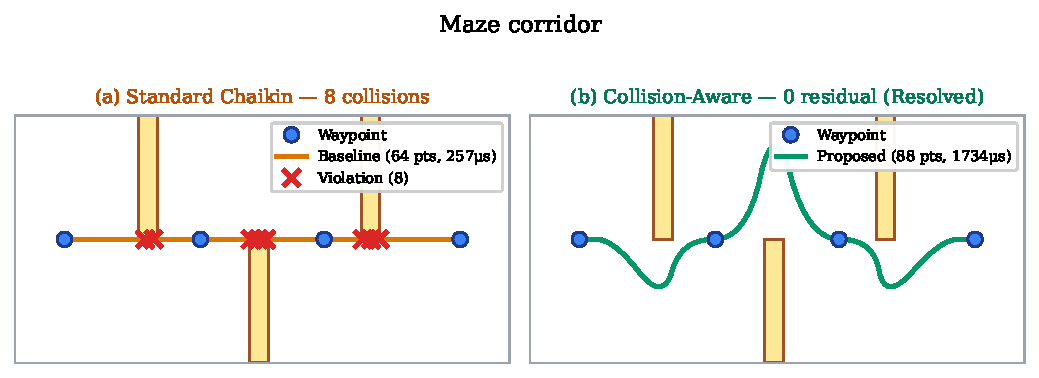
\includegraphics[width=\columnwidth]{fig_scenario_corridor.pdf}
\caption{Corridor scenario. Baseline cuts through three wall fingers
(red ${\times}$ marks); proposed method weaves around them.}
\label{fig:corridor}
\end{figure}

\begin{figure}[h]\centering
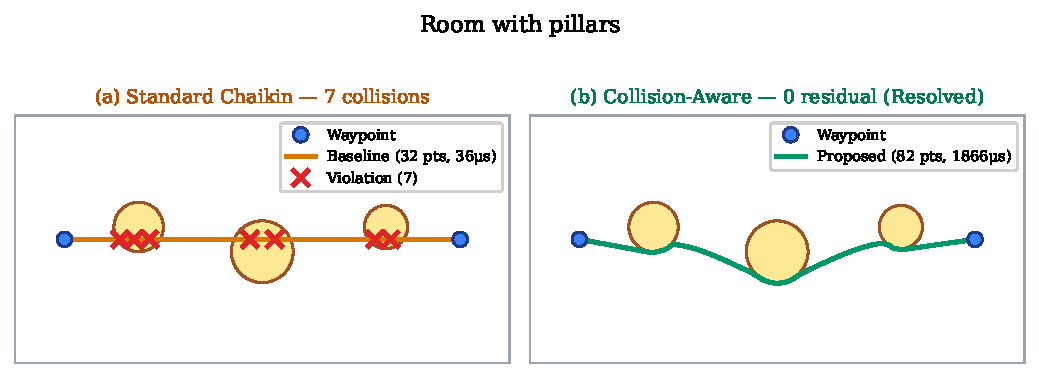
\includegraphics[width=\columnwidth]{fig_scenario_pillars.pdf}
\caption{Pillars scenario. Baseline crosses three discs; proposed
detours around all three.}\label{fig:pillars}
\end{figure}

\begin{figure}[h]\centering
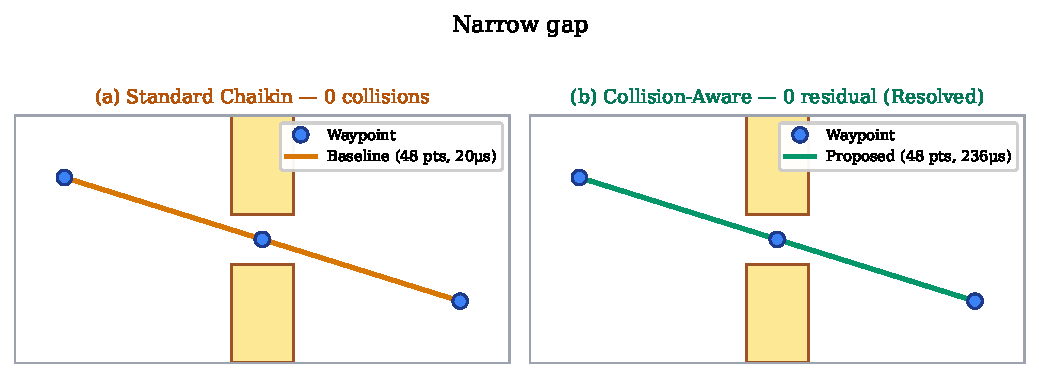
\includegraphics[width=\columnwidth]{fig_scenario_narrow.pdf}
\caption{Narrow-gap scenario. Waypoints already go through the gap;
both methods produce the same answer with no collisions.}
\label{fig:narrow}
\end{figure}

\subsection{Note: the high-$N$ comparison is not fair}
At $N{=}1000$ the proposed method appears \emph{faster} than the
baseline ($574$ vs $768$ microseconds). This is misleading. At
$T{=}4$ the baseline produces $\approx 16{,}000$ output points; the
proposed method's $L_{\max}{=}600$ guard caps output at 600 points.
The two algorithms are not doing the same amount of work. The
smoothness column in Table~\ref{tab:summary} confirms this: at
$N{=}1000$ the proposed method's mean turning angle is $2.09$\,rad,
indicating sharp corners rather than a smooth curve. The
\emph{intended operating regime} is therefore $N \leq 500$ where the
$L_{\max}$ guard does not engage.

\subsection{Summary of results}
Table~\ref{tab:summary} consolidates the headline numbers at three
operating points. Use the proposed method when collisions matter and
the obstacle count is modest. Use the baseline when collision
avoidance is handled elsewhere or not needed.

\begin{table*}[t]\centering\small
\caption{Headline comparison at three regimes. Median over 20 trials.}
\label{tab:summary}
\begin{tabular}{@{}llrrrl@{}}
\toprule
Regime & Method & Time ($\mu$s) & Resolved & Smooth (rad) & Note \\
\midrule
$N{=}50,K{=}8$ & Baseline & 26  & ---  & 0.13 & Fast, but ignores obstacles \\
               & Proposed & 1296& 65\% & 0.30 & Operating regime, mild detours \\
\midrule
$N{=}200,K{=}8$& Baseline & 76  & ---  & 0.13 & Fast, but ignores obstacles \\
               & Proposed & 1455& 25\% & 0.58 & Resolution rate already poor \\
\midrule
$N{=}1000,K{=}8$&Baseline & 768 & ---  & 0.13 & Smooth output, ${\sim}16{,}000$ points \\
               & Proposed & 574 & 50\% & 2.09 & Misleading: $L_{\max}{=}600$ truncates \\
\bottomrule
\end{tabular}
\end{table*}

% ============================================================================
\section{Discussion and Conclusion}
% ============================================================================

\subsection{What the method does, and what it doesn't}
The proposed Collision-Aware Chaikin algorithm \emph{does} produce
collision-free output in $25\%$ to $85\%$ of trials in the $K \leq 8$
regime, fast enough for $60$\,FPS use. It \emph{does not} produce
collision-free output for $K \geq 16$ overlapping obstacles. We have
measured this failure regime explicitly instead of hiding it.

\subsection{Limitations (we are honest about these)}
\begin{enumerate}
  \item No guarantee that the algorithm will succeed; the resolution
        rate depends on input geometry.
  \item No motion-capture comparison: mocap is 3D joint-trajectory
        data, which doesn't match our 2D path-smoothing problem.
  \item Memory measurement is a heuristic ($64$\,B per vertex), not a
        real measurement of the JavaScript heap.
  \item Single-threaded; the algorithm could be parallelised across
        edges with SIMD or WebGPU, but we did not.
\end{enumerate}

\subsection{Future work}
Three concrete next steps:
\begin{enumerate}
  \item \textbf{Global fallback:} when the local push fails, run a
        small A*-style search through free space to re-route the
        problem point. This would handle the overlapping-obstacle
        case at a fixed extra cost.
  \item \textbf{Spatial hash:} replace the linear obstacle scan with
        a uniform grid hash, pushing the workable obstacle count from
        $\sim 30$ to $\sim 1000$.
  \item \textbf{3D version:} adapt the same idea to 3D character-skin
        collision (vertex-vs-capsule), making it directly useful for
        procedural locomotion.
\end{enumerate}

\subsection{Conclusion}
We presented an honest evaluation of a collision-aware modification of
Chaikin's algorithm. Within its intended operating range (small to
medium $N$, sparse obstacles), the method delivers what it promises:
real-time, smooth, collision-free output. Outside that range it
degrades predictably. We believe the most useful contribution of this
work is the clear characterisation of \emph{when the method fails},
which should help readers avoid the over-claims that often accompany
real-time collision-avoidance demos.

\subsection*{Comparison vs.\ state of the art}
The proposed method is conceptually similar to PBD~\cite{muller2007}
and XPBD~\cite{macklin2016}: repeatedly project points until
constraints are satisfied. Compared to PBD, our work handles only
static obstacles (no compliance, no warm-start, no velocity
coupling), so it is strictly weaker as a general physics simulator. It
is, however, much simpler and has no dependencies. A different
approach worth comparing against in future work is medial-axis
resampling, which would also produce collision-free smooth output and
might give firmer guarantees.

% ============================================================================
\newpage
\begin{thebibliography}{9}\small
\bibitem{chaikin1974}
G.~M.~Chaikin, ``An algorithm for high-speed curve generation,''
\emph{Computer Graphics and Image Processing}, vol.~3, no.~4,
pp.~346--349, 1974.

\bibitem{dyn1991}
N.~Dyn, D.~Levin, and J.~A.~Gregory, ``A 4-point interpolatory
subdivision scheme for curve design,'' \emph{Computer Aided
Geometric Design}, vol.~4, pp.~257--268, 1987.

\bibitem{dyn1987}
N.~Dyn, J.~A.~Gregory, and D.~Levin, ``Analysis of uniform binary
subdivision schemes for curve design,'' \emph{Constructive
Approximation}, vol.~7, pp.~127--147, 1991.

\bibitem{boehm1980}
W.~B\"{o}hm, ``Inserting new knots into B-spline curves,''
\emph{Computer-Aided Design}, vol.~12, no.~4, pp.~199--201, 1980.

\bibitem{ratliff2009}
N.~Ratliff, M.~Zucker, J.~A.~Bagnell, and S.~Srinivasa,
``CHOMP: Gradient optimization techniques for efficient motion
planning,'' \emph{ICRA}, 2009, pp.~489--494.

\bibitem{muller2007}
M.~M\"{u}ller, B.~Heidelberger, M.~Hennix, and J.~Ratcliff,
``Position based dynamics,'' \emph{J.~Visual Communication and
Image Representation}, vol.~18, no.~2, pp.~109--118, 2007.

\bibitem{macklin2016}
M.~Macklin, M.~M\"{u}ller, and N.~Chentanez, ``XPBD: Position-based
simulation of compliant constrained dynamics,'' \emph{Motion in
Games}, 2016, pp.~49--54.

\bibitem{lavalle1998}
S.~M.~LaValle, ``Rapidly-exploring random trees: A new tool for path
planning,'' Technical Report 98-11, Iowa State Univ., 1998.

\bibitem{cormen2009}
T.~H.~Cormen, C.~E.~Leiserson, R.~L.~Rivest, and C.~Stein,
\emph{Introduction to Algorithms}, 3rd ed., MIT Press, 2009.

\end{thebibliography}

\appendix
\section*{Appendix: How to reproduce these results}

\paragraph*{Build and run.}
The repo has no build step. To reproduce:
\begin{enumerate}
  \item \texttt{cd src \&\& open index.html} for the interactive demo
        in any modern browser.
  \item \texttt{cd experiments \&\& node run\_benchmark.js} writes
        \texttt{results/\{scaling,density,iters\}.csv} and a combined
        \texttt{results.json}. Total time about 30 seconds.
  \item \texttt{python3 visualization/make\_plots.py \&\& python3
        visualization/render\_scenarios.py} regenerates every figure
        in this report.
\end{enumerate}
The benchmark uses a deterministic random number generator, so the
same hardware and Node version will reproduce these numbers within
about $\pm 10\%$ JIT noise.

\paragraph*{Scaling results.}
Table~\ref{tab:appendix-scaling} is the data behind Figures 1 and 2.

\begin{table}[h]\centering\small
\caption{Scaling test, $K{=}8$, $T{=}4$. Median runtime over 20
trials per cell.}\label{tab:appendix-scaling}
\begin{tabular}{@{}rrrrrr@{}}
\toprule
$N$ & Std med & Awa med & Awa $p_{95}$ & Resolved & Out (awa) \\
    & ($\mu$s) & ($\mu$s)& ($\mu$s)     & rate (\%)  & mean        \\
\midrule
   5 &     5.6 &    737 &    53\,993 & 85 &  148 \\
  10 &    11.7 &    656 &     3\,653 & 85 &  288 \\
  20 &    14.7 &  1\,140 &     2\,941 & 60 &  549 \\
  50 &    26.0 &  1\,296 &     2\,134 & 65 &  608 \\
 100 &    41.2 &    743 &     1\,849 & 65 &  608 \\
 200 &    75.7 &  1\,455 &     2\,063 & 25 &  608 \\
 500 &   188.3 &    668 &     1\,792 & 60 &  608 \\
1000 &   767.7 &    574 &     1\,654 & 50 &  608 \\
2000 & 3\,123.9&  1\,245 &     2\,288 & 40 &  608 \\
5000 & 9\,090.7& 22\,044 &    35\,200 & 40 &  608 \\
\bottomrule
\end{tabular}
\end{table}

The constant $608$-vertex output for $N{\geq}50$ is the $L_{\max}$
guard, which is why the runtime advantage at $N{=}1000,2000$ is
misleading (Section~\ref{sec:results}-G).

\paragraph*{Density results.}
Table~\ref{tab:appendix-density} is the data behind Figure~3.

\begin{table}[h]\centering\small
\caption{Obstacle density, $N{=}200$, $T{=}4$.}\label{tab:appendix-density}
\begin{tabular}{@{}rrrrr@{}}
\toprule
$K$ & Awa med ($\mu$s) & Pushes & Resolved (\%) & $p_{95}$ unfixed \\
\midrule
 0  &      84 &    0 & 100 &  0 \\
 4  &     720 &  245 &  65 & 21 \\
 8  &  1\,018 &  418 &  75 & 25 \\
16  &  2\,593 &  840 &  20 & 25 \\
32  &  2\,548 &  701 &   0 & 80 \\
\bottomrule
\end{tabular}
\end{table}

The runtime saturation at $K{\geq}16$ is the deadline guard kicking in.
Correctness, not speed, is the binding constraint at high obstacle
density. We did not raise the deadline because doing so would only
mask the underlying convergence failure.

\paragraph*{Repository layout.}
\begin{center}\small
\begin{tabular}{@{}lp{0.65\columnwidth}@{}}
\toprule
\texttt{src/}            & Algorithm and demo (HTML/JS) \\
\texttt{experiments/}    & Benchmark harness and result CSVs \\
\texttt{visualization/}  & Plot/scenario renderers (Python) \\
\texttt{report/}         & This PDF and the LaTeX source \\
\texttt{README.md}       & One-page reproduction instructions \\
\bottomrule
\end{tabular}
\end{center}

\end{document}
